\documentclass[aspectratio=169]{beamer}

\usepackage{amsmath}
\usepackage{fontspec}
\usepackage{tikz}

\setsansfont{Liberation Sans}
\usefonttheme{professionalfonts}
\usetheme{Copenhagen}
\setbeamertemplate{navigation symbols}{}
\setbeamertemplate{footline}[frame number]

\AtBeginSection{
  \begin{frame}[plain]
    \centering
    \vfill
    {\usebeamerfont{title}\usebeamercolor[fg]{structure}
      \Huge\insertsectionhead\par}
    \vfill
  \end{frame}
}

\title{Neural Network and Back Propagation from Scratch}
\author{}
\date{}

\begin{document}

\begin{frame}[plain]
  \titlepage
\end{frame}

\section{Intro}

\begin{frame}{The Original Goal}
  The original goal came from pure curiosity:

  \begin{quote}
    Build the smallest possible implementation of a neural network model.
  \end{quote}

  I wanted to understand how little code and machinery a working model
  actually needs.

  At first, this sounded like a concrete engineering task.
\end{frame}

\begin{frame}{Why the Goal Is Ill-Posed}
  The goal described what to build, but not what should count as success.

  \begin{itemize}
    \item A network no better than a coin flip is still technically a model.
    \item If accuracy is 80\%, should we continue to 81\%, 82\%, or 99\%?
    \item Quality alone ignores training time and computational cost.
    \item A model that outperforms all state-of-the-art models combined after
      trillions of years of training is not a useful result.
  \end{itemize}

  \begin{block}{A well-posed goal needs constraints}
    Define a target metric, a resource budget, and a stopping rule.
  \end{block}
\end{frame}

\begin{frame}[fragile]{Naive Algorithm: Brute-Force Selection}
  \small
  \textbf{Definitions:} $W$ is a neural network, $D$ is a dataset, and
  $L(W, D)$ is a loss to minimize. The function \texttt{rand\_net()} returns
  a random neural network.

\begin{verbatim}
best = rand_net()
for i = 1 to 1000:
    n1 = rand_net()
    if L(n1, D) < L(best, D):
        best = n1
\end{verbatim}

  Sample many random networks and keep the one with the lowest loss.

  This may produce accuracy slightly above chance. But once it does, should we
  stop?
\end{frame}

\begin{frame}[fragile]{{\normalsize Naive Algorithm №2: Random Local Search}}
  \small
\begin{verbatim}
best = rand_net()
step = 0.001
for i = 1 to 1000:
    g = rand_net() * step
    if L(best + g, D) < L(best, D):
        best = best + g
\end{verbatim}

  Instead of replacing the whole network, perturb its weights and accept only
  changes that reduce the loss.

  \begin{alertblock}{What changed?}
    The search procedure improved, but the objective did not become clearer.
  \end{alertblock}
\end{frame}

\section{Gradient Descent}

\begin{frame}{One Parameter, One Loss Curve}
  \begin{columns}[c]
    \begin{column}{0.43\textwidth}
      Consider a neural network with a single parameter $w_1$.

      For a fixed dataset $D$, its loss is now a function of one variable:

      \begin{equation*}
        \ell(w_1) = L(w_1, D).
      \end{equation*}

      Training becomes a geometric problem: find the lowest point on this
      two-dimensional graph.
    \end{column}
    \begin{column}{0.51\textwidth}
      \centering
      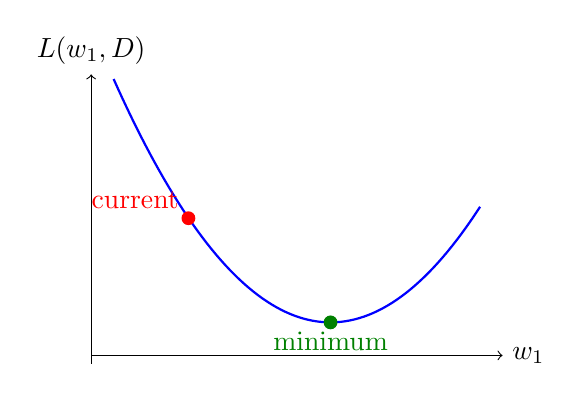
\begin{tikzpicture}[x=0.95cm, y=1.05cm]
        \draw[->] (-2.5, 0) -- (3, 0) node[right] {$w_1$};
        \draw[->] (-2.5, -0.1) -- (-2.5, 3.4)
          node[above] {$L(w_1, D)$};
        \draw[thick, blue, domain=-2.2:2.7, samples=80]
          plot (\x, {0.35 * (\x - 0.7)^2 + 0.4});
        \fill[red] (-1.2, 1.66) circle (2.5pt)
          node[above left] {current};
        \fill[green!50!black] (0.7, 0.4) circle (2.5pt)
          node[below] {minimum};
      \end{tikzpicture}
    \end{column}
  \end{columns}
\end{frame}

\begin{frame}{From a Limit to a Numerical Derivative}
  Define $f(w_1) = L(w_1, D)$. The derivative is the limit of the slope
  between two increasingly close points:

  \begin{columns}[T]
    \begin{column}{0.47\textwidth}
      \begin{block}{Exact derivative}
        \begin{equation*}
          f'(w_1)
          =
          \lim_{h \to 0}
          \frac{f(w_1 + h) - f(w_1)}{h}.
        \end{equation*}
      \end{block}
    \end{column}
    \begin{column}{0.47\textwidth}
      \begin{block}{Finite difference}
        \begin{equation*}
          h = \texttt{1e-5}
        \end{equation*}
        \begin{equation*}
          g_1
          =
          \frac{L(w_1 + h, D) - L(w_1, D)}{h}.
        \end{equation*}
      \end{block}
    \end{column}
  \end{columns}

  For a small, finite $h$, $g_1 \approx f'(w_1)$: it estimates how quickly
  the loss grows when $w_1$ increases.
\end{frame}

\begin{frame}{One Gradient Descent Step}
  \begin{columns}[c]
    \begin{column}{0.58\textwidth}
      \centering
      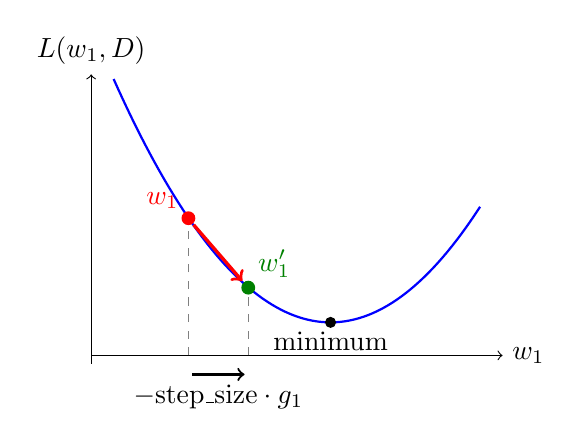
\begin{tikzpicture}[x=0.95cm, y=1.05cm]
        \draw[->] (-2.5, 0) -- (3, 0) node[right] {$w_1$};
        \draw[->] (-2.5, -0.1) -- (-2.5, 3.4)
          node[above] {$L(w_1, D)$};
        \draw[thick, blue, domain=-2.2:2.7, samples=80]
          plot (\x, {0.35 * (\x - 0.7)^2 + 0.4});
        \draw[dashed, gray] (-1.2, 0) -- (-1.2, 1.66);
        \draw[dashed, gray] (-0.4, 0) -- (-0.4, 0.82);
        \draw[->, very thick, red] (-1.13, 1.58) -- (-0.48, 0.9);
        \draw[->, thick] (-1.15, -0.23) -- (-0.45, -0.23)
          node[midway, below] {$-\text{step\_size} \cdot g_1$};
        \fill[red] (-1.2, 1.66) circle (2.5pt)
          node[above left] {$w_1$};
        \fill[green!50!black] (-0.4, 0.82) circle (2.5pt)
          node[above right] {$w_1'$};
        \fill[black] (0.7, 0.4) circle (2pt)
          node[below] {minimum};
      \end{tikzpicture}
    \end{column}
    \begin{column}{0.36\textwidth}
      \begin{block}{Update rule}
        \begin{equation*}
          \texttt{step\_size = 0.01}
        \end{equation*}
        \begin{equation*}
          w_1' = w_1 - \text{step\_size} \cdot g_1
        \end{equation*}
      \end{block}

      $g_1$ points uphill, so the minus sign moves the parameter downhill.

      Recompute the derivative at the new point and repeat.
    \end{column}
  \end{columns}
\end{frame}

\begin{frame}[fragile]{From One Parameter to Many}
  \small
  Let $W = (w_1, \ldots, w_n)$ and collect all partial derivatives in a vector
  $G$.

\begin{verbatim}
base_loss = L(W, D)
G = zeros(n)
for i = 1 to n:
    W_probe = W
    W_probe[i] += h
    G[i] = (L(W_probe, D) - base_loss) / h

W = W - step_size * G
\end{verbatim}

  {\footnotesize
    $^{*}$ We evaluate $L$ independently for every parameter: once for each
    perturbed parameter, plus one shared evaluation of \texttt{base\_loss}.
  }
\end{frame}

\begin{frame}{Why Numerical Gradients Do Not Scale}
  With a sufficiently small $h$, finite differences can train the network.
  The problem is speed.

  \begin{block}{Cost of one training step}
    For each of the $N$ parameters, compute the loss $L$ once:
    \begin{equation*}
      \text{total work}
      \approx
      \underbrace{N}_{\text{number of parameters}}
      \times
      \underbrace{L}_{\text{one full loss evaluation}}.
    \end{equation*}
    Thus, one gradient step needs approximately $N$ evaluations of $L$.
  \end{block}

  \begin{alertblock}{The bottleneck}
    Networks that do anything non-trivial have a huge number of parameters.
    One training step therefore requires a huge number of evaluations of $L$.
  \end{alertblock}
\end{frame}

\section{Optimizing Gradient Descent}

\begin{frame}[fragile]{Stochastic Gradient Descent}
  Instead of computing the loss on the entire dataset at once, split the
  dataset into smaller batches:

  \begin{equation*}
    D \quad\longrightarrow\quad B_1, B_2, \ldots, B_k.
  \end{equation*}

  Compute the gradient on one batch, update the parameters, and continue with
  the next batch.

  \begin{block}{Training loop}
\begin{verbatim}
for batch in batches:
    G = compute_gradient(L, W, batch)
    W -= step_size * G
\end{verbatim}
  \end{block}

  Here, \texttt{compute\_gradient(L, W, batch)} means
  $\nabla_W L(W, \text{batch})$: the gradient of the batch loss with respect
  to $W$.
\end{frame}

\begin{frame}{Back Propagation}
  Here we develop an intuitive understanding of back propagation.

  \begin{block}{Intuition}
    Back propagation is a way to compute gradients using the chain rule.
  \end{block}

  Understanding back propagation is critical to understanding how neural
  networks learn.
\end{frame}

\begin{frame}{Chain Rule}
  \small
  \begin{columns}[T]
    \begin{column}{0.43\textwidth}
      Recall the derivative of a function of one variable:
      \begin{equation*}
        f'(x)
        =
        \lim_{h \to 0}
        \frac{f(x+h)-f(x)}{h}.
      \end{equation*}
    \end{column}
    \begin{column}{0.51\textwidth}
      For several inputs, keep the other inputs fixed:
      \begin{align*}
        f(x,y)=xy
          &:& \frac{\partial f}{\partial x}=y,
          && \frac{\partial f}{\partial y}=x, \\
        f(x,y)=x+y
          &:& \frac{\partial f}{\partial x}=1,
          && \frac{\partial f}{\partial y}=1.
      \end{align*}
    \end{column}
  \end{columns}

  \begin{block}{Definition}
    The chain rule computes the derivative of a composition of two or more
    functions from their individual derivatives. If $f(x)=g(h(x))$, then
    \begin{equation*}
      f'(x)=g'(h(x))h'(x).
    \end{equation*}
  \end{block}
\end{frame}

\begin{frame}{Compound Expressions with the Chain Rule}
  Consider a more complicated expression composed of multiple functions:

  \begin{equation*}
    f(x,y,z)=(x+y)z.
  \end{equation*}

  Name the inner expression $q=x+y$. Then $f=qz$, and
  \begin{align*}
    \frac{\partial f}{\partial x}
      &= \frac{\partial f}{\partial q}
         \frac{\partial q}{\partial x}, \\
    \frac{\partial f}{\partial q} &= z,
    &\qquad
    \frac{\partial q}{\partial x} &= 1, \\
    \frac{\partial f}{\partial x}
      &= z \cdot 1 = z.
  \end{align*}

  \vfill
  {\footnotesize
    A trillion-parameter LLM, written as one formula at just $1$ mm per
    parameter, would be about $2.6$ Earth--Moon distances long.
  }
\end{frame}

\begin{frame}{A Computation Graph}
  Back propagation works on any computation graph. A neural network is only
  one particular case.

  For this example, use the simplest possible loss: $L(l_3)=l_3$.

  \centering
  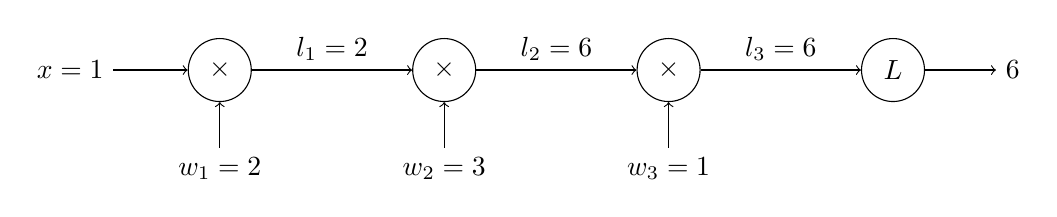
\begin{tikzpicture}[x=0.95cm, y=1cm]
    \node (x) at (0,0) {$x=1$};
    \node[draw, circle, minimum size=0.8cm] (mul1) at (2,0) {$\times$};
    \node[draw, circle, minimum size=0.8cm] (mul2) at (5,0) {$\times$};
    \node[draw, circle, minimum size=0.8cm] (mul3) at (8,0) {$\times$};
    \node[draw, circle, minimum size=0.8cm] (loss) at (11,0) {$L$};
    \node (result) at (12.6,0) {$6$};
    \node (w1) at (2,-1.25) {$w_1=2$};
    \node (w2) at (5,-1.25) {$w_2=3$};
    \node (w3) at (8,-1.25) {$w_3=1$};
    \draw[->] (x) -- (mul1);
    \draw[->] (w1) -- (mul1);
    \draw[->] (mul1) -- node[above] {$l_1=2$} (mul2);
    \draw[->] (w2) -- (mul2);
    \draw[->] (mul2) -- node[above] {$l_2=6$} (mul3);
    \draw[->] (w3) -- (mul3);
    \draw[->] (mul3) -- node[above] {$l_3=6$} (loss);
    \draw[->] (loss) -- (result);
  \end{tikzpicture}

  \vspace{0.5em}
  First, evaluate the graph from left to right.
\end{frame}

\begin{frame}{Gradient for One Weight}
  \small
  \begin{equation*}
    g_2
    = \frac{\partial L}{\partial w_2}
    = \frac{\partial l_2}{\partial w_2}
      \frac{\partial L}{\partial l_2}.
  \end{equation*}

  \begin{columns}[T]
    \begin{column}{0.46\textwidth}
      \begin{block}{Known from left to right}
        Since $l_2=l_1w_2$,
        \begin{equation*}
          \frac{\partial l_2}{\partial w_2}=l_1=2.
        \end{equation*}
        The value $l_1$ was stored while evaluating the graph.
      \end{block}
    \end{column}
    \begin{column}{0.46\textwidth}
      \begin{block}{Known from right to left}
        \begin{equation*}
          \frac{\partial L}{\partial l_2}=1.
        \end{equation*}
        We computed this derivative earlier because back propagation moves
        from right to left.
      \end{block}
    \end{column}
  \end{columns}

  \begin{alertblock}{Combine both values}
    \centering
    $g_2=l_1\frac{\partial L}{\partial l_2}=2\cdot1=2.$
  \end{alertblock}
\end{frame}

\section{From Biological Neuron to Neural Network}

\begin{frame}{From Biology to Computation}
  \begin{columns}[T]
    \begin{column}{0.48\textwidth}
      \begin{block}{Biological neuron}
        \centering
        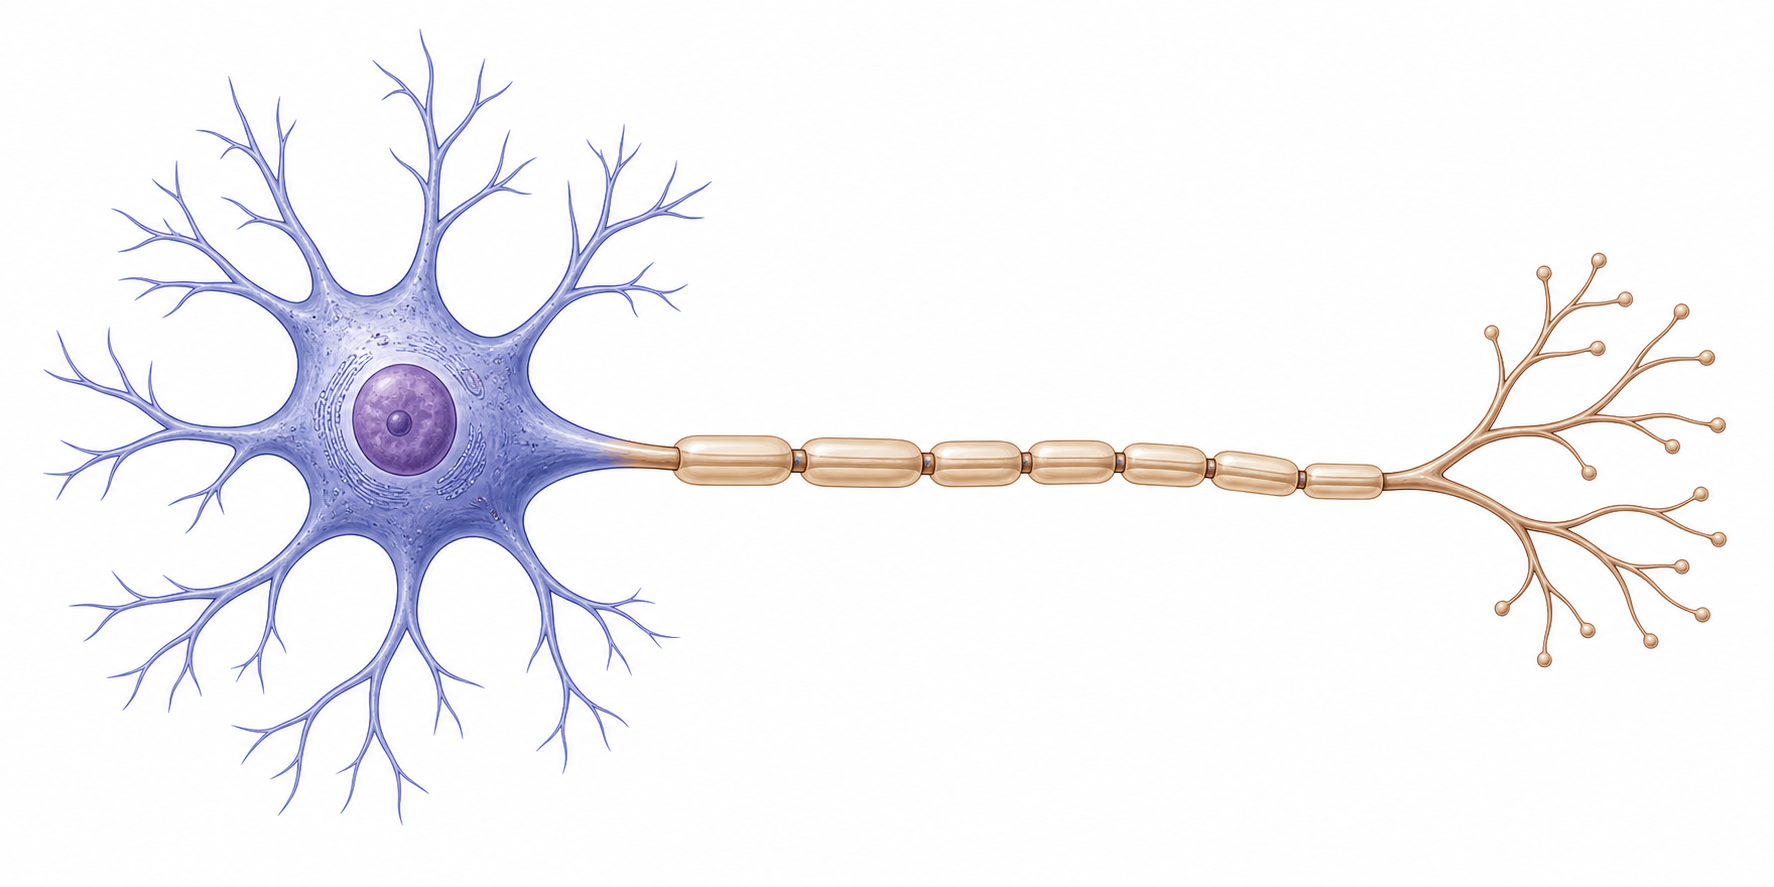
\includegraphics[width=\linewidth]{assets/biological-neuron.png}
      \end{block}

      Receives signals through dendrites and sends one signal through the
      axon.
    \end{column}
    \begin{column}{0.46\textwidth}
      \begin{block}{Computational model}
        \centering
        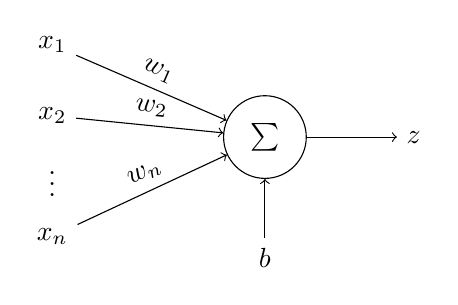
\begin{tikzpicture}[x=0.9cm, y=0.9cm]
          \node (x1) at (0,1.5) {$x_1$};
          \node (x2) at (0,0.5) {$x_2$};
          \node (dots) at (0,-0.35) {$\vdots$};
          \node (xn) at (0,-1.2) {$x_n$};
          \node[draw, circle, minimum size=1.05cm] (sum) at (3,0.2)
            {$\sum$};
          \node (bias) at (3,-1.5) {$b$};
          \node (z) at (5.1,0.2) {$z$};
          \draw[->] (x1) -- node[above, sloped] {$w_1$} (sum);
          \draw[->] (x2) -- node[above, sloped] {$w_2$} (sum);
          \draw[->] (xn) -- node[above, sloped] {$w_n$} (sum);
          \draw[->] (bias) -- (sum);
          \draw[->] (sum) -- (z);
        \end{tikzpicture}
      \end{block}

      Computes one number from numeric inputs and weights.
    \end{column}
  \end{columns}

  \vspace{0.4em}
  {\footnotesize\itshape
    The artificial neuron is an analogy, not a detailed simulation of a
    living cell.
  }
\end{frame}

\begin{frame}{A Neuron as a Computation}
  The graph multiplies every input by its weight, adds the results, and adds a
  bias:

  \begin{block}{Scalar form}
    \begin{equation*}
      z
      = w_1x_1 + w_2x_2 + \cdots + w_nx_n + b.
    \end{equation*}
  \end{block}

  Collect the inputs and weights into vectors:
  \begin{equation*}
    x = (x_1, \ldots, x_n),
    \qquad
    w = (w_1, \ldots, w_n).
  \end{equation*}

  \begin{alertblock}{Vector form}
    \begin{equation*}
      z = w^\mathsf{T}x + b.
    \end{equation*}
  \end{alertblock}
\end{frame}

\begin{frame}{Same Network, Two Representations}
  \small
  \begin{columns}[T]
    \begin{column}{0.40\textwidth}
      \begin{block}{Computation graph: $2 \to 3 \to 2$}
        \centering
        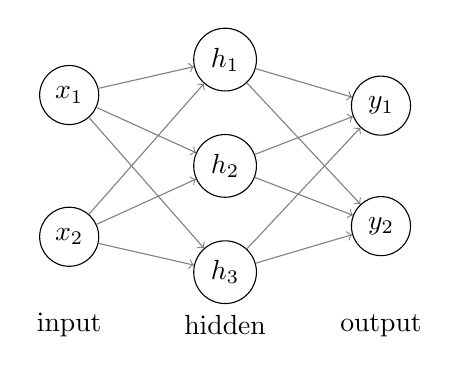
\begin{tikzpicture}[
          x=0.9cm,
          y=0.9cm,
          neuron/.style={draw, circle, minimum size=0.75cm},
        ]
          \node[neuron] (x1) at (0,1) {$x_1$};
          \node[neuron] (x2) at (0,-1) {$x_2$};
          \node[neuron] (h1) at (2.2,1.5) {$h_1$};
          \node[neuron] (h2) at (2.2,0) {$h_2$};
          \node[neuron] (h3) at (2.2,-1.5) {$h_3$};
          \node[neuron] (y1) at (4.4,0.85) {$y_1$};
          \node[neuron] (y2) at (4.4,-0.85) {$y_2$};
          \foreach \i in {1,2} {
            \foreach \j in {1,2,3} {
              \draw[->, gray] (x\i) -- (h\j);
            }
          }
          \foreach \i in {1,2,3} {
            \foreach \j in {1,2} {
              \draw[->, gray] (h\i) -- (y\j);
            }
          }
          \node at (0,-2.25) {input};
          \node at (2.2,-2.25) {hidden};
          \node at (4.4,-2.25) {output};
        \end{tikzpicture}
      \end{block}
    \end{column}
    \begin{column}{0.54\textwidth}
      \begin{block}{The same network as matrices}
        \begin{equation*}
          \begin{bmatrix}h_1 \\ h_2 \\ h_3\end{bmatrix}
          =
          \underbrace{
            \begin{bmatrix}
              w_{11} & w_{12} \\
              w_{21} & w_{22} \\
              w_{31} & w_{32}
            \end{bmatrix}
          }_{W_1\; (3 \times 2)}
          \begin{bmatrix}x_1 \\ x_2\end{bmatrix}
          + b_1
        \end{equation*}

        \begin{equation*}
          \begin{bmatrix}y_1 \\ y_2\end{bmatrix}
          =
          \underbrace{
            \begin{bmatrix}
              v_{11} & v_{12} & v_{13} \\
              v_{21} & v_{22} & v_{23}
            \end{bmatrix}
          }_{W_2\; (2 \times 3)}
          \begin{bmatrix}h_1 \\ h_2 \\ h_3\end{bmatrix}
          + b_2
        \end{equation*}
      \end{block}
    \end{column}
  \end{columns}

  Each row of a matrix contains all incoming weights of one neuron.
\end{frame}

\begin{frame}{Without ReLU, Three Layers Become One}
  \small
  \begin{block}{Three consecutive matrix multiplications}
    \centering
    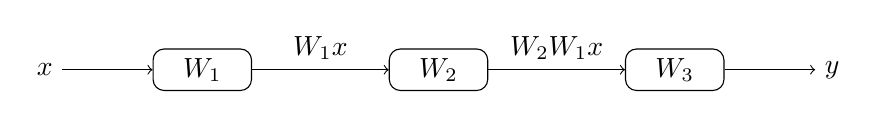
\begin{tikzpicture}[x=1cm, y=1cm]
      \node (x) at (0,0) {$x$};
      \node[draw, rounded corners, minimum width=1.25cm] (w1) at (2,0)
        {$W_1$};
      \node[draw, rounded corners, minimum width=1.25cm] (w2) at (5,0)
        {$W_2$};
      \node[draw, rounded corners, minimum width=1.25cm] (w3) at (8,0)
        {$W_3$};
      \node (y) at (10,0) {$y$};
      \draw[->] (x) -- (w1);
      \draw[->] (w1) -- node[above] {$W_1x$} (w2);
      \draw[->] (w2) -- node[above] {$W_2W_1x$} (w3);
      \draw[->] (w3) -- (y);
    \end{tikzpicture}

    \vspace{-0.3em}
    \begin{equation*}
      y = W_3\bigl(W_2(W_1x)\bigr) = (W_3W_2W_1)x.
    \end{equation*}
  \end{block}
  \vspace{-0.3em}

  \begin{block}{One equivalent matrix multiplication}
    \centering
    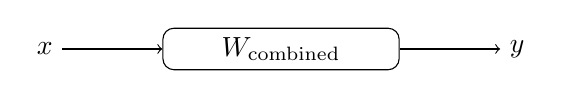
\begin{tikzpicture}[x=1cm, y=1cm]
      \node (x) at (0,0) {$x$};
      \node[draw, rounded corners, minimum width=3cm] (wc) at (3,0)
        {$W_{\text{combined}}$};
      \node (y) at (6,0) {$y$};
      \draw[->] (x) -- (wc);
      \draw[->] (wc) -- (y);
    \end{tikzpicture}
    \qquad
    $W_{\text{combined}} = W_3W_2W_1$.
  \end{block}
  \vspace{-0.3em}

  \begin{alertblock}{ReLU prevents this collapse}
    With $\operatorname{ReLU}(z)=\max(0,z)$ between the matrices,
    $y=W_3\operatorname{ReLU}(W_2\operatorname{ReLU}(W_1x))$ cannot generally
    be reduced to one matrix multiplication.
  \end{alertblock}
\end{frame}

\begin{frame}[fragile]{One Layer in Pseudocode}
  \small
  One layer is a matrix--vector product, a bias, and a nonlinearity:

  \begin{block}{Matrix-style pseudocode}
\begin{verbatim}
def layer(x, W, b):
    z = W @ x + b
    output = maximum(z, 0)
    return output
\end{verbatim}
  \end{block}

  \begin{equation*}
    \underbrace{x}_{n\times 1}
    \xrightarrow{\quad W\in\mathbb{R}^{m\times n}\quad}
    \underbrace{Wx+b}_{m\times 1}
    \xrightarrow{\quad \operatorname{ReLU}\quad}
    \underbrace{\max(0,Wx+b)}_{m\times 1}.
  \end{equation*}
\end{frame}

\begin{frame}[fragile]{Forward Pass Through Hidden Layers}
  \small
  Apply the same computation to every hidden layer and store each activation:

  \begin{block}{Simplified from \texttt{NN::forward\_pass}}
\begin{verbatim}
def forward(x, weights, biases):
    activations = [x]

    for layer in range(len(weights)):
        z = weights[layer] @ x + biases[layer]
        x = relu(z)
        activations.append(x)

    return activations
\end{verbatim}
  \end{block}

  \vspace{0.3em}
  {\footnotesize
    \textbf{Why store activations?} Back propagation reuses each layer's input
    to compute its weight gradient.
  }
\end{frame}

\begin{frame}[fragile]{Back Propagation Through Hidden Layers}
  \footnotesize
  Start with the loss derivative and visit the layers in reverse order:

  \begin{block}{Simplified from \texttt{NN::back\_propagation}}
\begin{verbatim}
def backpropagation(target, prediction, weights, activations):
    d = prediction - target
    for layer in reversed(range(len(weights))):
        previous = activations[layer]
        bias_grads[layer] += d
        for row in range(len(d)):
            for col in range(len(previous)):
                weight_grads[layer][row][col] += d[row] * previous[col]
        d = transpose(weights[layer]) @ d
        d *= relu_derivative(previous)
\end{verbatim}
  \end{block}

  {\scriptsize
    $\operatorname{ReLU}'(a)$ is $1$ where $a>0$, otherwise $0$.\par
  }
\end{frame}

\begin{frame}[fragile]{One Mini-Batch Training Step}
  \footnotesize
  \begin{block}{Simplified from \texttt{NN::train}}
\begin{verbatim}
def train(batch_inputs, batch_targets):
    for x, target in zip(batch_inputs, batch_targets):
        activations = forward(x, weights, biases)
        prediction = activations[-1]
        backpropagation(target, prediction,
                        weights, activations)
    apply_grads()
\end{verbatim}
  \end{block}
\end{frame}

\begin{frame}{Thank You!}
  \centering
  \vfill
  {\Huge Thank you for your attention!}

  \vspace{2em}
  \begin{block}{Source code}
    \centering
    {\scriptsize
      \url{https://github.com/kvladsrc/gym/blob/main/neural_network/nn_lib/nn_lib.cc}
    }
  \end{block}
  \vfill
\end{frame}

\end{document}
